\documentclass[aspectratio=43]{beamer}
\usetheme{Berlin}

\usepackage[czech]{babel}
\usecolortheme{dolphin}
\usepackage{graphicx}
\usepackage{dirtree}
\usepackage{listings}
\usepackage[T1]{fontenc}
\usepackage{lmodern}
\usepackage[utf8]{inputenc}
\usepackage{caption}
\usepackage{bbding}
\usepackage{xurl}
\usepackage{scrextend}
\usepackage{minted}
\usepackage{appendixnumberbeamer}

\captionsetup{labelformat=empty}

\beamertemplatenavigationsymbolsempty
\defbeamertemplate*{title page}{customized}[1][]
{
	\usebeamerfont{title}\inserttitle\par
	\usebeamerfont{subtitle}\usebeamercolor[fg]{subtitle}\insertsubtitle\par
	\bigskip
	\usebeamerfont{author}\insertauthor\par
	\usebeamerfont{institute}\insertinstitute\par
	\usebeamerfont{date}\insertdate\par
	\usebeamercolor[fg]{titlegraphic}\inserttitlegraphic
}

\hypersetup{unicode}
\hypersetup{breaklinks=true}

%%% Please fill in basic information on your thesis, which will be automatically
%%% inserted at the right places. You need to replace ... by real data.

% Type of your thesis:
%	"bc" for Bachelor's
%	"mgr" for Master's
%	"phd" for PhD
%	"rig" for rigorosum
% "sem" for semestral
\def\ThesisType{bc}


\def\ThesisTitle{Surveillance FMCW Radar}

\def\ThesisTitleShort{Surveillance FMCW Radar}

\def\ThesisAuthor{Havránek Kryštof}

\def\MontSubmitted{TODO}

\def\YearSubmitted{2024}

\def\Institution{Czech Technical University in Prague}

\def\Faculty{Faculty of Electrical Engineering}

\def\DepartmentType{Department}

\def\Department{Department of Electromagnetic Field}

\def\Supervisor{Ing. Viktor Adler, Ph.D}

\def\SupervisorsDepartment{Department of Electromagnetic Field}

\def\StudyProgramme{Elektronika a komunikace}

\def\Dedication{%
Dedication.
}

\def\Abstract{%
	TODO
}

% 3 to 5 keywords (recommended) separated by \sep
% Keywords are useful for indexing and searching for the theses by topic.
\def\ThesisKeywords{%
	TODO
}

% If any of your metadata strings contains TeX macros, you need to provide
% a plain-text version for use in XMP metadata embedded in the output PDF file.
% If you are not sure, check the generated thesis.xmpdata file.
\def\AuthorXMP{\ThesisAuthor}
\def\TitleXMP{\ThesisTitle}
\def\KeywordsXMP{\ThesisKeywords}
\def\AbstractXMP{\Abstract}

% If your abstracts are long and do not fit in the infopage, you can make the
% fonts a bit smaller by this setting. (Also, you should try to compress your abstract more.)
\def\InfoPageFont{}
%\def\InfoPageFont{\small}  % uncomment to decrease font size

% If you are studing in a Czech programme, you also need to provide metadata in Czech:
% (in English programmes, this is not used anywhere)

\def\ThesisTitleCS{Přehledový FMCW radar}
\def\DepartmentCS{Katedra elektromagnetického pole}
\def\DepartmentTypeCS{Katedra}
\def\SupervisorsDepartmentCS{Katedra elektromagnetického pole}
\def\StudyProgrammeCS{Elektronika a komunikace}

\def\ThesisKeywordsCS{%
	TODO
}

\def\AbstractCS{%
	TODO
}




\title{\ThesisTitle}
\subtitle{\Department}
\author{Havránek Kryštof }
\date{5th December 2024}
\institute{ČVUT-FEL}
\setbeamertemplate{sidebar right}{}
\setbeamertemplate{footline}{%
\hfill\textbf{\insertframenumber{}/\inserttotalframenumber} \hspace{0.01cm} \vspace{0.1cm}}
\setbeamerfont{footnote}{size=\tiny}

\begin{document}

\begin{frame}[plain]
	\maketitle
\end{frame}

\clearpage
\setcounter{framenumber}{0}



\begin{frame}[fragile]
\section{Introduction}
  \frametitle{Goal of the thesis}
  \begin{itemize}
    \item Design a two-axis rotary platform purpose build for radar-based applications
    \item Cost effective platform -- off-the-shelf components
    \item Simple control mechanism
    \item Timely and deterministic movement
  \end{itemize}
\end{frame}

\begin{frame}[fragile]
  \frametitle{Hardware}
  \section{Hardware}
  \begin{figure}[!htb]
    \begin{minipage}{0.48\textwidth}
      \begin{itemize}
        \item 3D printed parts
        \item Use of a slipring
        \item Optical endstops for homing
        \item ESP32 + basic stepper driver
      \end{itemize}
    \end{minipage}\hfill
    \begin{minipage}{0.48\textwidth}
      \centering
      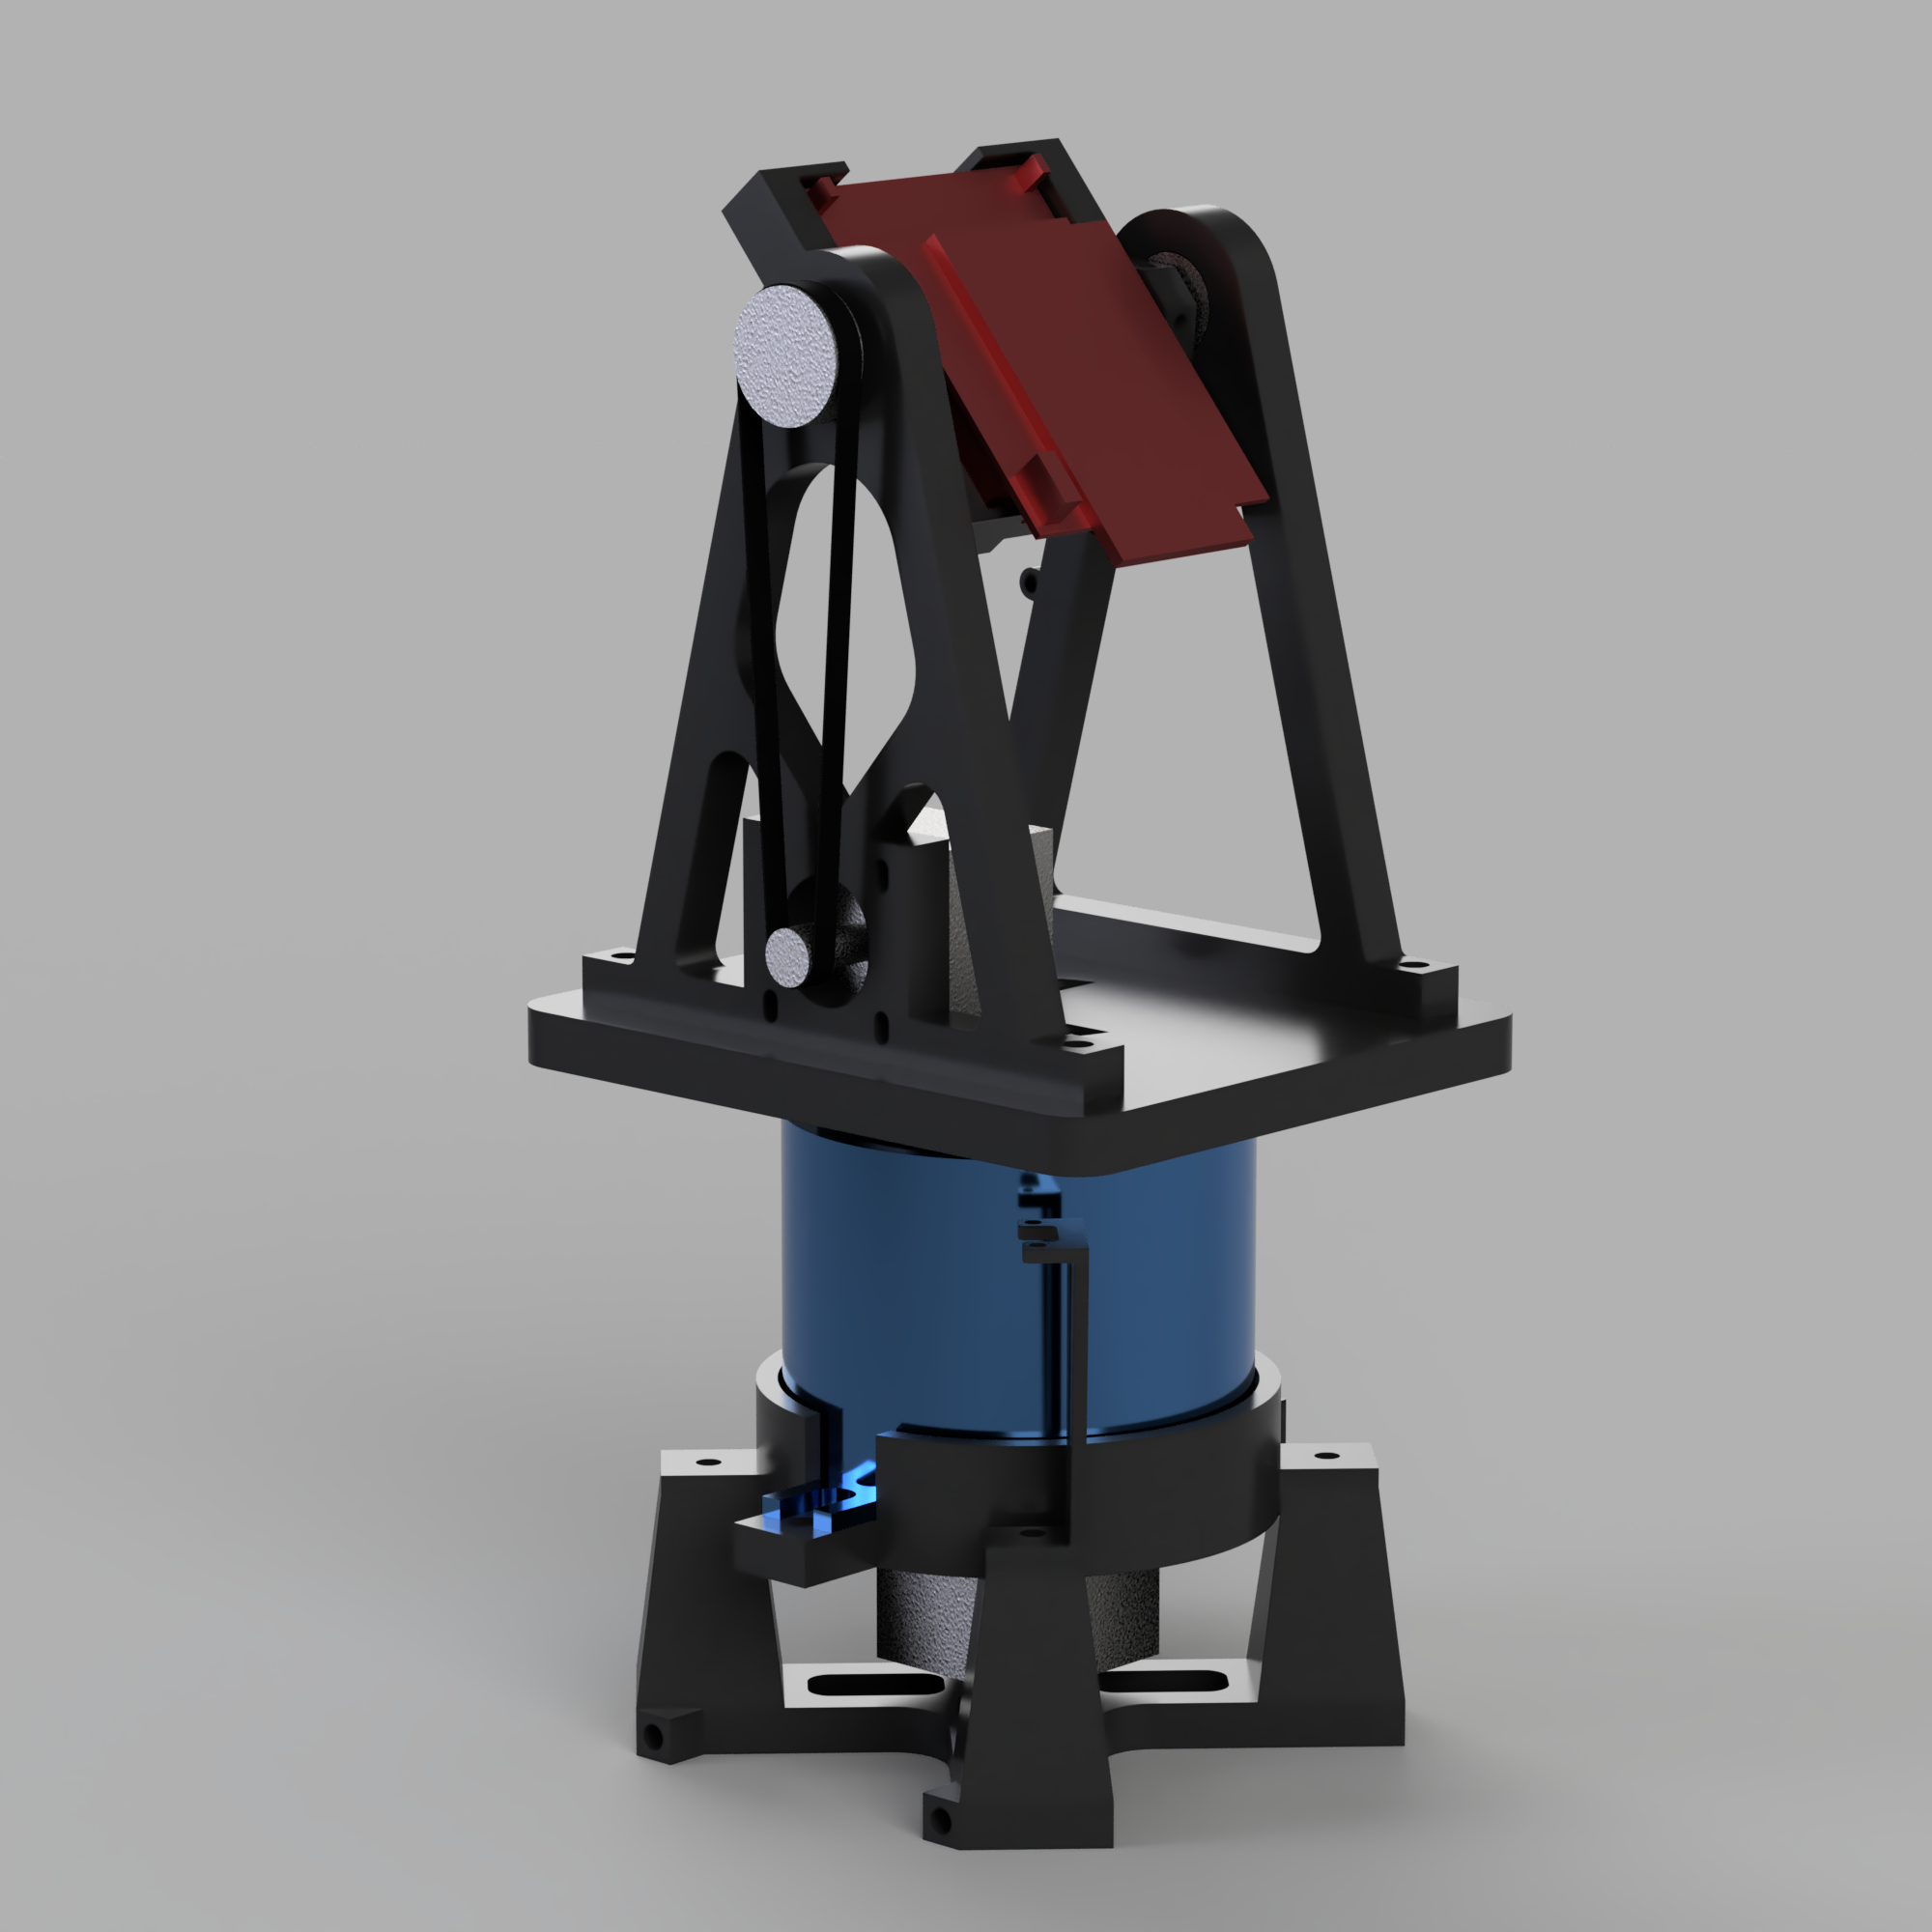
\includegraphics[height=\linewidth]{../img/whole_assembly_2.png}
      \caption{3D render}
    \end{minipage}
  \end{figure}
\end{frame}

\begin{frame}[fragile]
  \frametitle{Software}
  \section{Software}
	\begin{figure}[!htb]
		\begin{minipage}{0.48\textwidth}
			\begin{itemize}
    \item Three-layer command processing architecture
    \item Prescheduling of tasks
    \item Programming environment -- declaration of movement command sequences
    \item Controlled with G-code over serial
			\end{itemize}
		\end{minipage}\hfill
		\begin{minipage}{0.48\textwidth}
			\centering
			\includegraphics[height=\linewidth, trim = 30mm 30mm 30mm 25mm, ]{./memoize.memo.dir/BDE417D794BE8D061E9010BC0D77F984-E778DCCCB8AAB0BBD3F6CFEEFD2421F8.pdf}
		\end{minipage}
	\end{figure}
\end{frame}

\begin{frame}[fragile]
  \frametitle{Conclusion}
  \section{Conclusion}
  \begin{itemize}
    \item Speed control with $\epsilon=-0.004\%$
    \item Imperceivable delays during command switching
    \item Easy integration into other projects
    \item Practical, affordable alternative to existing commercial systems
  \end{itemize}
\end{frame}

\end{document}
